\chapter{The Red Thread for this thesis}
\textbf{Always connect software engineering, mobile analytics, and reliability.}

Implicit feedback mechanisms provided by various forms of usage analytics (mobile analytics). Some of these are instigated by developers, others are instigated by library and/or platform providers. The feedback mechanisms are used to identify probable issues in mobile apps where the development team then choose to address at least a subset of those issues with the aim of improving the quality-in-use~\citep{} of future releases of that app. 

The research is mainly empirical owing to the nature of usage analytics and the analytics tools which thrive on volume and realism. Mixed methods were used to expand the research, for instance by using static analysis into how developers use and maintain remote logging in the codebases of their Android apps. The case studies include examples where the researcher was:
\begin{enumerate}
    \item embedded: an active participant integrated into the project team,
    \item coach: of an existing team of developers who applied the concepts,
    \item interviewer: of various development teams to learn of their practices and results,
    \item analyst/observer: performing static analysis of opensource code repositories.
\end{enumerate}

The research includes several aspects seldom studied owing to the challenges of obtaining the case studies, for instance from behind the curtain in commercial projects with over a million users, and from sources again seldom visible to researchers \emph{i.e.} of mobile analytics for real-world mobile apps.

\newpage

\begin{figure}
    \centering
    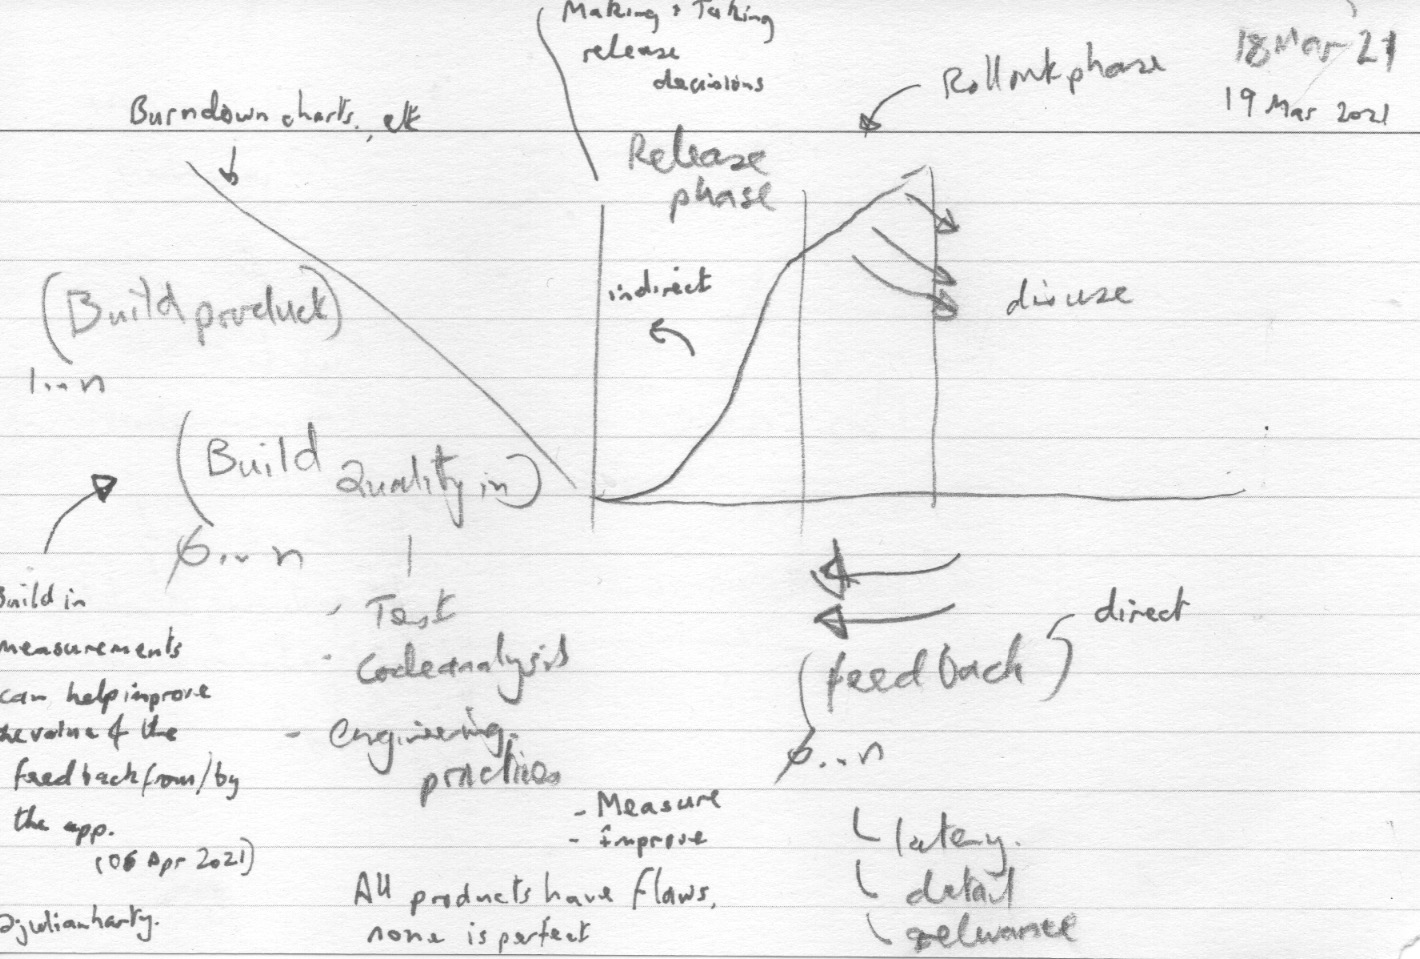
\includegraphics[width=15cm]{images/rough-sketches/Red-Thread-Rough-Sketch.jpeg}
    \caption{Red Thread Illustration for this thesis}
    \label{fig:red-thread-for-this-thesis}
\end{figure}

For any given release of a mobile app there are three phases:
\begin{enumerate}
    \item Building the product: which may incorporate practices and tools intended to ship a `quality product'. Some teams also incorporate logging and reporting to help measure the behaviours of the app in use, post release.
    \item The Release: For some projects this may be as simple as uploading a new binary and making it fully available. For others they may incorporate decisions and mechanisms to make each release with the aim of de-risking any undesirable/adverse effects of the new release.
    \item Live, where end users install and use the release of the app.
\end{enumerate}

Figure~\ref{fig:red-thread-for-this-thesis} illustrates these three phases together with some of the dynamics \emph{e.g.} of rollout and disuse of a release, and of feedback from whatever sources that the development teams can choose to pay attention to and apply.

Developers can choose when they will pay attention to the analytics; they can also choose the extent they wish to integrate analytics into their apps. Significant data is available for minimal effort, nonetheless the development teams who choose to invest in analytics are able to reap better and more relevant results. There are risks and responsibilities of the effects of collecting data and performing analysis on that data, practices outstrip legislation. It remains possible for sensitive findings to be discovered through the use of mobile analytics, nonetheless the ethical challenges are not unique to mobile analytics.

This research found that developers are able to materially improve the stability/reliability~\footnote{Stability is a term used by Google when they describe their Android Vitals service which is incorporated into Google Play Console. It includes measures of crashes and ANRs. An overview of Android Vitals is available online from various Google and Android sources including~\citep{android_vitals_overview_2019, android_vitals_best_practices}.}
%
of their mobile apps when they use the results of mobile analytics to assess the stability/reliability, identify groups of failures, triage the failures, and address the ones they decide to action. Where project teams stop paying attention to this process the failure rate increases of their new releases - the apps tend to entropy and failure.

Diligent developers and development teams can materially improve the stability/reliability of their apps through applying good coding, design and architecture patterns. Even these practices do not guarantee the releases will always be trouble-free. By paying ongoing attention to analytics during development, testing, and the rollout of releases flaws can be identified before the release reaches the majority of the userbase and teams can ameliorate the effects of many of the flaws.

\newpage 

\begin{figure}
    \centering
    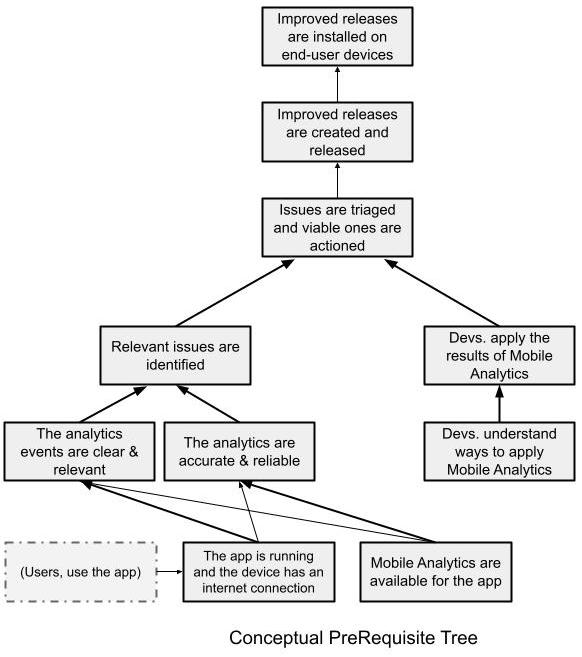
\includegraphics[width=15cm]{images/my/Conceptual_prereq_tree_Applying_Theory_of_Constraints_to_using_Mobile_Analytics_to_improve_Mobile_Apps.jpeg}
    \caption{Using Mobile Analytics to improve Mobile Apps ToC Conceptual PreRequisites Tree}
    \label{fig:using-toc-cpt-using-mobile-analytics-to-improve-mobile-apps}
\end{figure}

Figure~\ref{fig:using-toc-cpt-using-mobile-analytics-to-improve-mobile-apps} illustrates a conceptual pre-requisite tree (applying Theory of Constraints, see~\citep{goldratt2017_necessary_but_not_sufficient, lepore1999_deming_and_goldratt, scheinkopf1999_thinking_for_a_change}). 


[4] Joorabchi, Mona Erfani, Ali Mesbah, and Philippe Kruchten. "Real challenges in mobile app development." Empirical Software Engineering and Measurement, 2013 ACM/IEEE International Symposium on 10 Oct. 2013: 15-24.


Many developers fail to address all the issues identified through use of mobile analytics and a key influence is their perceived ability to successfully address issues identified by the analytics. Furthermore, these issues are collectively only one of many demands for their time and attention. Human, organisational, and business factors all influence the extent mobile analytics is a) used and b) the results addressed. This research touches on both the mechanics of applying mobile analytics together with the `game' which are the higher-level human nature aspects which affect the application and the value of applying the mechanics. Figure~\ref{fig:the-mechanics-the-game} provides a simple illustration of the game and the mechanics.

\begin{figure}
    \centering
    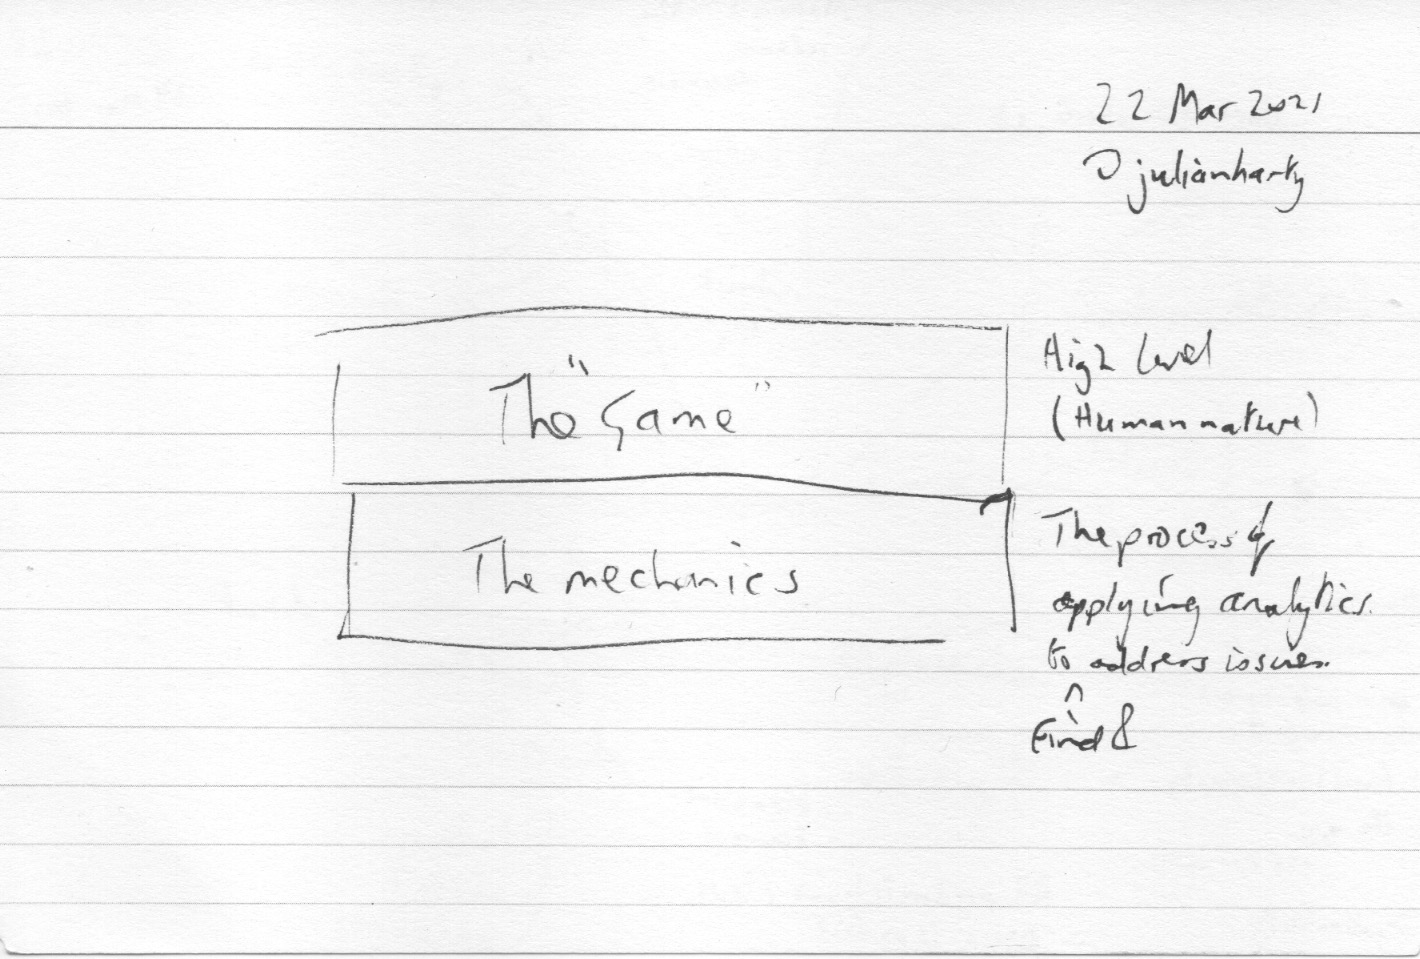
\includegraphics[width=15cm]{images/rough-sketches/The-Mechanics-The-Game.jpeg}
    \caption{The Mechanics and The Game of using Mobile Analytics}
    \label{fig:the-mechanics-the-game}
\end{figure}

Analytics providers have a major influence on the efficacy of the application of mobile analytics. There are limitations and flaws in the various tools this research has encountered regardless of their source (\emph{e.g.} in-house proprietary, opensource, free and paid-for commercial proprietary offerings). Nonetheless, flawed offerings are still able to be used to deliver improvements in the mobile apps. Specialised startups such as Iteratively aim to increase the coherence of embedded analytics (those embedded into the apps) while also increasing compliance. 
